%% manuscript produces a one-column, double-spaced document:
\documentclass[manuscript]{aastex}
%\documentclass[manuscript]{emulateapj}
%\documentclass[twocolumn]{article}
%\documentclass[twocolumn]{emulateapj}

%% preprint2 produces a double-column, single-spaced document:
%% Sometimes a paper's abstract is too long to fit on the
%% title page in preprint2 mode. When that is the case,
%% use the longabstract style option.

%% \documentclass[preprint2,longabstract]{aastex}

%% If you are submitting to a journal that translates manuscripts
%% into SGML, you need to follow certain guidelines when preparing
%% your macros. See the AASTeX v5.x Author Guide
%% for information.

\newcommand{\vdag}{(v)^\dagger}
\newcommand{\numt}{60}
\newcommand{\cii}{\ensuremath{\mathrm{C}\,\scriptstyle \mathrm{II}}}
\newcommand{\oi}{\ensuremath{\mathrm{O}\,\scriptstyle \mathrm{I}}}
\newcommand{\hi}{\ensuremath{\mathrm{H}\,\scriptstyle \mathrm{I}}}
\newcommand{\siIV}{\ensuremath{\mathrm{Si}\,\scriptstyle \mathrm{IV}}}

%% You can insert a short comment on the title page using the command below.

%%\slugcomment{Not to appear in Nonlearned J., 45.}

%% If you wish, you may supply running head information, although
%% this information may be modified by the editorial offices.
%% The left head contains a list of authors,
%% usually a maximum of three (otherwise use et al.).  The right
%% head is a modified title of up to roughly 44 characters.
%% Running heads will not print in the manuscript style.

\shorttitle{Using Limb Brightening for Transit Timing}
\shortauthors{Schlawin et al.}

%% This is the end of the preamble.  Indicate the beginning of the
%% paper itself with \begin{document}.

\begin{document}

%% LaTeX will automatically break titles if they run longer than
%% one line. However, you may use \\ to force a line break if
%% you desire.

\title{Double-U Light Curves:\\
Planetary Transits at Limb Brightened Wavelengths}

%% Use \author, \affil, and the \and command to format
%% author and affiliation information.
%% Note that \email has replaced the old \authoremail command
%% from AASTeX v4.0. You can use \email to mark an email address
%% anywhere in the paper, not just in the front matter.
%% As in the title, use \\ to force line breaks.

\author{E. Schlawin} 
\affil{Astronomy Department, Cornell University, Ithaca NY 14850}
\author{E. Agol}
\affil{Astronomy Department, University of Washington, Seattle, WA 98195}
\author{J. Lloyd}
\affil{Astronomy Department, Cornell University, Ithaca NY 14850}
\author{L. Walkowicz}
\affil{Astronomy Department,University of California at Berkeley,Berkeley, CA 94720}
\author{K. Covey\altaffilmark{1}}
\affil{Astronomy Department, Cornell University, Ithaca NY 14850}


%%\affil{Astronomy Department, Cornell University,
%%    Ithaca, NY 14853}

% PUT THIS BACK IN ONC YOU FIGURE OUT HOW TO MAKE IT NOT CONFLICT WITH TEXT
%\altaffiltext{1}{Hubble Fellow}

%% Mark off your abstract in the ``abstract'' environment. In the manuscript
%% style, abstract will output a Received/Accepted line after the
%% title and affiliation information. No date will appear since the author
%% does not have this information. The dates will be filled in by the
%% editorial office after submission.

\bibliographystyle{apj}

\begin{abstract}
\end{abstract}

%% Keywords should appear after the \end{abstract} command. The uncommented
%% example has been keyed in ApJ style. See the instructions to authors
%% for the journal to which you are submitting your paper to determine
%% what keyword punctuation is appropriate.

\keywords{extrasolar planets: transit timing --- stellar chromospheres}
%% Authors who wish to have the most important objects in their paper
%% linked in the electronic edition to a data center may do so by tagging
%% their objects with \objectname{} or \object{}.  Each macro takes the
%% object name as its required argument. The optional, square-bracket 
%% argument should be used in cases where the data center identification
%% differs from what is to be printed in the paper.  The text appearing 
%% in curly braces is what will appear in print in the published paper. 
%% If the object name is recognized by the data centers, it will be linked
%% in the electronic edition to the object data available at the data centers  
%%
%% Note that for sources with brackets in their names, e.g. [WEG2004] 14h-090,
%% the brackets must be escaped with backslashes when used in the first
%% square-bracket argument, for instance, \object[\[WEG2004\] 14h-090]{90}).
%%  Otherwise, LaTeX will issue an error. 

\section{Introduction}
Of the exoplanets so far discovered, more than \numt\ are known to
transit their host star. These planets, with their favorable orbital
alignment, reveal planetary radii, stellar radii and average
density. Even more information about their orbit can be gleaned from
the exact epoch at which they transit their host star. So called
transit timing variation (TTV) measurements
\citep{2005MNRAS.359..567A} (and cite more?) are designed to reveal
deviations from Keplerian elliptical motion due to the tug other
planets and satellites.

Previous transit timing has been done with optical and infrared
telescopes \citep{2004ApJ...613L.153A,2010A&A...510A.107M} (\& add
some more TTV papers?) Light curves for these kind of transits have a
sharp negative slope at ingress and a sharp positive slope at
egress. In the middle, they have a gradual concave up curvature due to limb darkening of the star.

We outline a method of observing that has the opposite curvature; some
wavelengths are limb brightened so the flux at these wavelengths goes
{\it up} mid-transit. This will occur for any optically thin
chromospheric or coronal emission line. Just as with a planetary
nebula, like the Ring Nebula, the limb of an optically thin shell of
gas is brighter at the edges. This is because the column density at
the limb is much larger at the limb than in the center. \footnote{Note
that this effect is different from what causes limb darkening.} As a
consequence, a transit curve will be ``W''-shaped, where the maximum
transit depth occurs at the stellar limbs.

\citet{assef} point out that limb brightening could be
very useful for detection of transits of giant planets. One advantage
to photometry in limb brightened wavelengths is that transits are
deeper overall than for both limb brightened and uniform disk
emission. This is because the planet cover a larger amount of the
emission. \citet{assef} approximate the limb brightened
star as a uniform ring of emission. With their approximation, the maximum depth
of the transit scales as $R_p/R_*$ instead of $(R_p/R_*)^2$,
as expected for a uniform disk.

We show in this paper that a more accurate limb brightened
approximation for the transit depth scales as $(R_p/R_*)^{3/2}$. In
$\mathsection$\ref{labl:chromlcurve} we calculate the expected limb
brightened light curve for an optically thin emission line and compare
this to UV images of the Sun. In $\mathsection$\ref{labl:stactv}, we
discuss the effects of stellar activity on these observations. We
compare the expected transit timing precision for UV photometry with
optical photometry in $\mathsection$\ref{labl:sn} and list targets
suitable for UV photometry in $\mathsection$\ref{labl:targ}. We also
outline several possibilities for chromospheric science in
$\mathsection$\ref{labl:cscience}.

\section{Limb Brightened Curves} \label{labl:chromlcurve}

\subsection{Chromospheric light curve: thin-shell approximation}
\label{labl:thinshell}
If the scale-height of the chromosphere, $h$, is much smaller than the
size of the planet and star, $R_p, R_*$, then we can treat the
chromosphere as a geometrically thin hemisphere of emission.  This
limit has the problem that at the edge of the shell, the surface
brightness will be infinite; this is an example classic fold-caustic.
However, when one integrates the surface brightness over area, the
total flux is finite, and thus this still proves to be a useful
approximation.

%However, rather than integrating over surface brightness to compute
%the transit depth, 
%the depth of transit is simply the area of the 
%hemisphere that is blocked by the planet, 

We can estimate this maximum depth of transit as follows from
Figure \ref{fig01}.  When the planet touches the edge of the star 
(second contact), as shown from an edge-on viewpoint in this figure,
then the length of the arc of the long axis of the shadow is
$R_*\theta$.  Now, the diameter of the planet is given by 
$2 R_p \approx R_*(1-\cos{\theta}) \approx \frac{1}{2} R_* \theta^2$,
where the latter approximation is valid for $\theta \ll 1$.
Solving for $\theta$, we find $\theta = 2\sqrt{R_p/R_*}$, so to
be valid we require $R_p/R_* \ll 1/4$.  Now, we can approximate
the shadow as an ellipse which will have a minor axis of $R_p$
and a major axis of $R_*\theta$, so we can approximate the
area of the shadow as $A_t = \pi \sqrt{R_pR_*} R_p$.  Thus,
the maximum depth of transit is given by 
\begin{equation} \label{depth_anal}
{A_t \over \pi R_*^2} = \frac{1}{2} \left({R_p \over R_*}\right)^{3/2}.
\end{equation}
Note that this is a different scaling than that given in \citet{assef} who did not consider the fold-caustic nature of a chromospheric
transits.

This has the remarkable consequence that the depth of a chromospheric
transit does not decline as much with the radius of the planet as 
a transit of a uniform disk.  A chromospheric transit has a maximum
depth that is $\frac{1}{2} \left({R_* \over R_p}\right)^{1/2}$
times deeper than the maximum transit depth of a uniform disk;
thus smaller planets have an advantage to be observed at
chromospheric wavelengths, as emphasized by \citet{assef}.

\begin{figure}
%\centerline{\psfig{figure=Chromospheric_shadow.eps,width=4in}}
%\includegraphics[trim = 1in 6in 2in 0.5in,clip,width=3
%  in]{Chromospheric_shadow.eps}
\includegraphics[width=\textwidth]{Chromospheric_shadow.eps}
\caption{Edge-on view of area of shadow cast by the planet
at the edge of the star.}
\label{fig01}
\end{figure}

We can compute the light curve for $h=0$ in terms of elliptic integrals.
Let $b$ be the impact parameter of center of the planet relative to
the center of the star in units of the radius of the star, as
seen by an observer.  Let $a = A_t/R_*^2$ be the dimensionless transit
area, and $f(b,p)=1-\frac{a}{2\pi}$ is the transit light curve.
For $b > 1+p$, there is no transit, so $a=0$.
For $1+p > b > 1-p$, the planet straddles the edge of the star, and
depth of transit is:
\begin{eqnarray}\label{ingress}
a&=&2\pi\Theta(p-b)+{1\over \sqrt{bp}}\left[{b+p\over b-p}\Pi(n,k)-4bpE(k)-(1-2p(b+p))K(k)\right] \cr
k&=&\sqrt{1-(b-p)^2\over 4bp}, \cr 
n&=&(b-p)^{-2}-1,
\end{eqnarray}
where $K(k)$, $E(k)$, and $\Pi(n,k)$ are complete Legendre elliptic 
integrals of the first, second, and third kinds, and $\Theta(x)$ is
the Heaviside step function.

For $0 < b < 1-p$, the planet is fully contained within the disk of the star,
and the transit depth is:
\begin{eqnarray}\label{disk}
a&=&2\pi\Theta(p-b)+{k\over \sqrt{bp}}\left[{b+p\over b-p}\Pi(n,k)-4bpk^{-2}E(k)
             +(p^2-b^2)K(k)\right],\cr
k&=&\sqrt{4bp\over 1-(b-p)^2},\cr
n&=&4bp/(b-p)^2.
\end{eqnarray}

These formulae are difficult to evaluate numerically at 
$b=p$ and $b=1-p$ due to the divergenced of $K(1)$ and $\Pi(n,1)$,
; the divergences cancel out analytically, but routines that
evaluate the elliptic integrals diverge.  However, these locations
are a set of measure zero, and thus should almost never be encountered
when modeling data.

\subsection{Dependence on planet size}

Figure \ref{fig02} plots the transit light curves for planet of
two different sizes, $p=0.02$ and $p=0.04$ versus the planet-star
separation, $b$.  The analytic estimate does a remarkably good
job in predicting the maximum depth of a chromospheric transit,
which means that the chromospheric depth is 3.5 and 2.5 times
deeper for the two planets, respectively.  Although the smaller
planet has a transit depth that is 25\% of the larger planet's
transit depth for a star without limb-darkening, the maximum 
chromospheric transit depth for the smaller planet is 35\% that 
of the larger planet, and is nearly as deep as the transit of 
the larger planet.  Note that the duration of ingress/egress 
scales with the size of the planet in both cases.  

There are several consquences of the deeper transit depth:
(1) transit-timing precision is higher for a chromospheric
transit than for a non-limb darkened transit by a factor of
$\sim p^{-1/2}$ assuming the same signal-to-noise for
both light curves; (2) the larger depth and short duration
of the chromospheric transit can make detection of giant
planets transiting sub-giant stars greater possibility;
and (3) since the advantage of chromospheric transits
over continuum transits grows as $\frac{1}{2}p^{-1/2}$,
the chromospheric transits have a greater advantage for
transit detection of small planets. For instance
for $p=0.01$, the chromospheric transit is $5\times$
deeper, which is appropriate for Earth-Sun transits
or giant planets transiting a $10R_\odot$ star.

Although the considerations in this section apply
for the geometrically-thin shell approximation,
we now show that this also applies when one considers
the physical extent of the chromosphere.

\begin{figure}
%\centerline{\psfig{figure=comp_size.eps,width=4in}}
%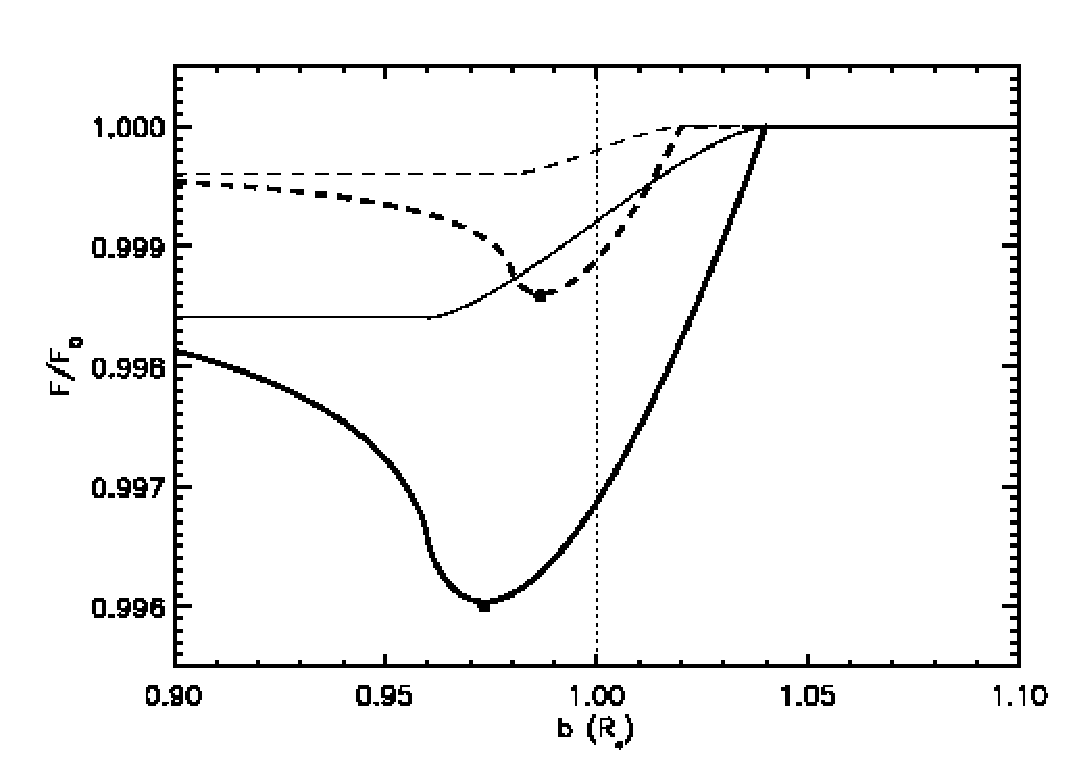
\includegraphics[trim = 1in 6in 2in 0.5in,clip,width=3
%  in]{comp_size.eps}
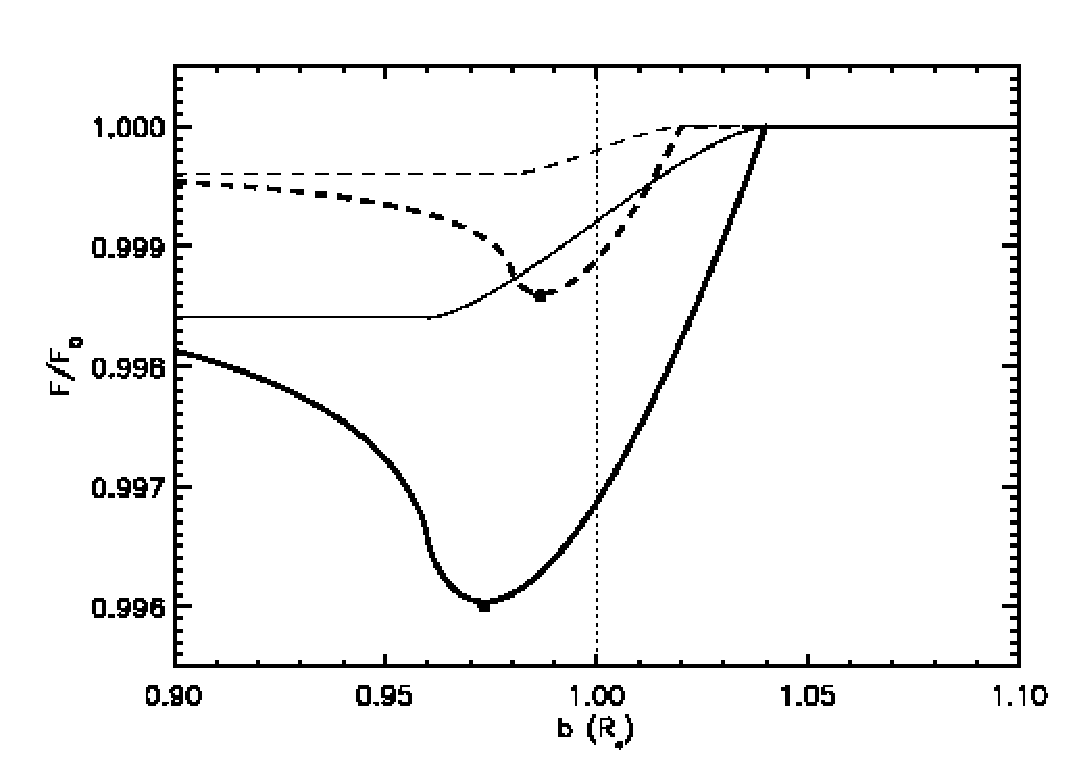
\includegraphics[width=\textwidth]{comp_size.eps}
\caption{Transit light curve depth near ingress/egress 
for $p=0.04$ (solid lines) and $p=0.02$ (dashed lines).
The thick lines show a chromospheric transit, while the 
thin lines show a transit of a source of uniform brightness.
The vertical dotted line marks the edge of the star.
The large dots show the prediction of the analytic
estimate of the maximum chromospheric transit depth\ref{depth_anal}.}
\label{fig02}
\end{figure}

\subsection{Isothermal chromosphere models}

In the chromosphere the coronal approximation applies,
which means that every collisional excitation results
in cooling by optically-thin radiative emission.
If we take the chromosphere to be isothermal, then
the emissivity scales as the square of the density,
$\epsilon \propto \rho^2$.  For an isothermal chromosphere
in which $h \ll R_*$, the density should be exponential,
so $\epsilon \propto e^{-2 (r-R_*)/h}$ where $R_*$
now represents the base of the chromosphere where it
becomes optically-thick.

We computed the emission of this emissivity, which is plotted in
Figure \ref{fig03}.  Note the rather similar appearance to images of
the Sun's corona.  There is a discontinuity in surface brightness at
$b=1$ due to the opaque inner boundary of our model; at this point the
emissivity from beyond the midplane of the star is blocked, while for
slightly larger impact parameters we see the emissivity on the far
side of the star.  This feature is only present if there is a sharp
discontinuity in the opacity of the chromosphere.

\begin{figure}
%%\centerline{\psfig{figure=chromosphere_disk.eps,width=3in} \psfig{figure=chromosphere_surface_brightness.eps,width=3in}}
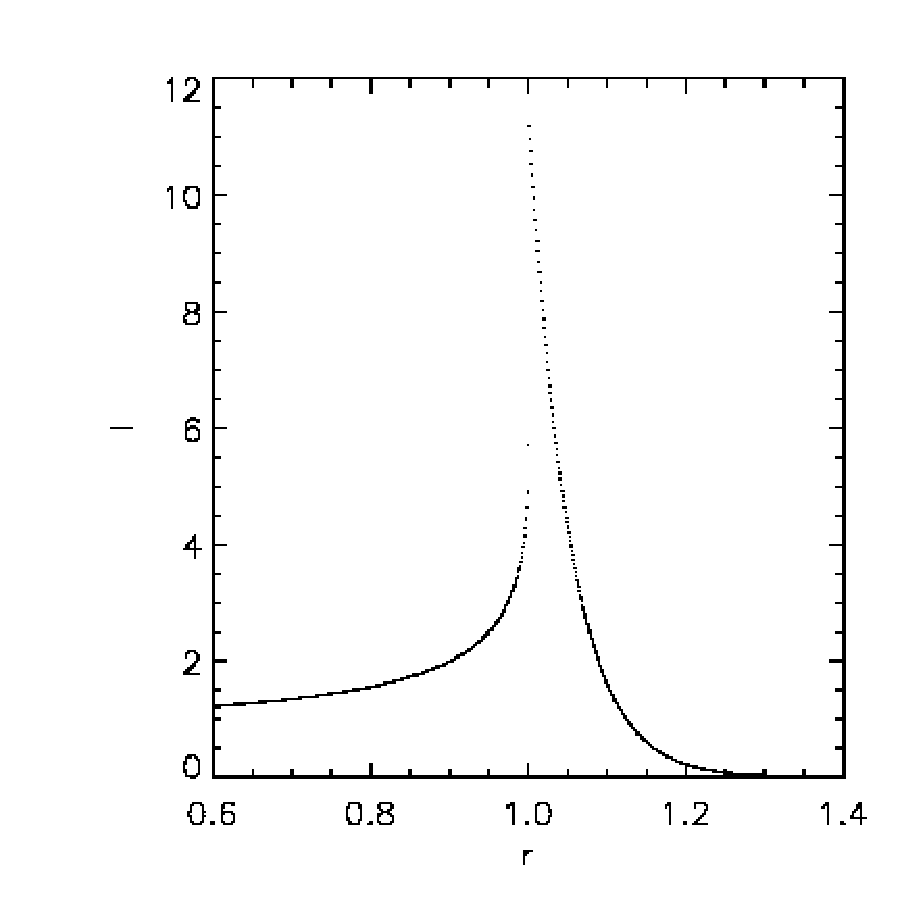
\includegraphics[width=\textwidth]{chromosphere_surface_brightness.eps}
\caption{Isothermal chromospheric model. Left hand panel shows a simulated 2D
image for $h=0.1R_*$, while the right hand panel shows the
surface brightness plotted in the radial direction near
the limb for $h=0.1R_*$ (solid line) and $h=0.01R_*$
(dashed line).  The surface brightness for the geometrically-thin
approximation is not plotted as it is nearly indistinguishable from 
the $h=0.01R_*$ surface brightness on this scale.}
\label{fig03}
\end{figure}

We have computed transit lightcurves using this brightness
profile, and an example of the results is shown in Figure
\ref{fig04}.  As the scale height shrinks, the light
curve approaches that of the geometrically-thin model.
For $h > p$, the transit starts further from the disk of
the star due to the more extended surface brightness profile
of the star.  Since the chromosphere is more diffuse for
larger values of $h$, the transit depth is smaller and
broader.  For $h < p$ and $h \rightarrow 0$, the light curve 
starts  to approach that of the geometrically-thin limit.
The transit depth is slightly deeper for $h<p$ since the
emissivity is somewhat brighter near the limb due to
the fact that we can see the emission from the far side
of the star which is invisible when $h=0$.  The maximum
depth depends on both $p$ and $h$; for instance, for 
$p=0.1$, the maximum depth is 7\% deeper than for
the thin-shell depth at $h \approx 0.2 p$, while
for $p=0.02$, the maximum depth occurs at $h=0.01$
and is 18\% deeper than for the thin-shell depth.
There is a cusp in the curves at $b=1-p$ (i.e.\ second or third 
contact) due to the discontinuity in surface brightness at 
$b=1$.

\begin{figure}
%\centerline{\psfig{figure=lc_h.1_p.1.eps,width=3in}

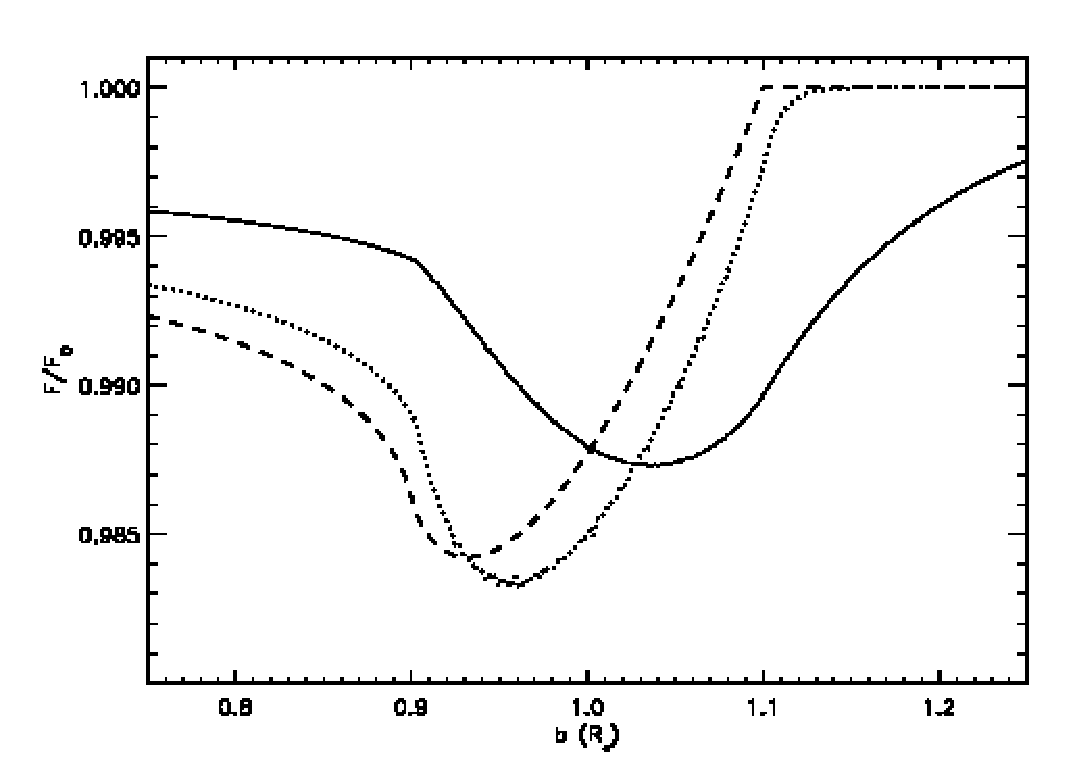
\includegraphics[width=0.5\textwidth]{lc_h.1_p.1.eps}
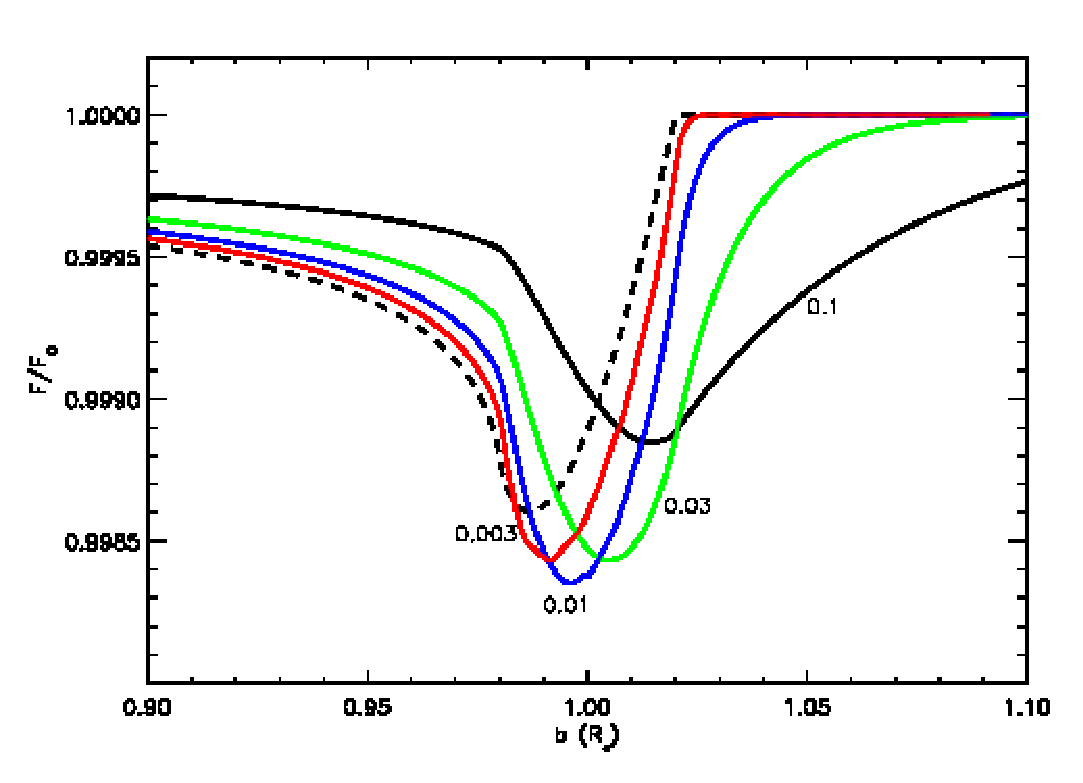
\includegraphics[width=0.5\textwidth]{plot_3d_p.02.eps}
%\psfig{figure=plot_3d_p.02.eps,width=3in}}
\caption{Chromospheric transit light curves for the
isothermal chromospheric model with $p=0.1$ (left) and
$p=0.02$ (right).   In the left panel, the
solid line is for $h=0.2$; the dotted line for $h=0.02$;
and the dashed line for $h=0$ (i.e.\ the geometrically-thin
chromosphereic model, equations \ref{ingress},\ref{disk}).
In the right panel, the curves are labelled by $h$:
$h=0.1$ (black), $h=0.03$ (green), $h=0.01$ (blue),
$h=0.003$ (red), and $h=0$ (black dashed).}
\label{fig04}
\end{figure}

\subsection{Comparison With Solar Images}

\section{Limb Brightened Lines}

-\\
Optically thin lines are the most limb-brightened
-\\
-\\
For M Stars in the Near UV, we'd be looking at 
-\\
- FeII, SiII lines from 2300 \AA\  to 2775 \AA\ 
-\\
- Don't include the optically thick MgII h and k lines at
$\sim$2800 \AA\ \citep{2007PASP..119...67H}
-\\
-\\

\subsection{Stellar Activity} \label{labl:stactv}
-\\
-    Starspots - are they a problem? \\
-\\
-    Compare Transit lifetime to flare lifetimes
-  Select and list more quiescent stars that would be good candidates


\subsection{Targets for UV Observations} \label{labl:targ}
- I think this is going to be M-dwarfs and giants \\
- stars where our method beats conventional photometry
-      Report GALEX fluxes \\
-   Possible telescopes - Swift, Hubble or GALEX \\

\subsection{Previous Observations of HD 209458b}

\citet{viddisc} observed HD 209458b with the STIS instrument and found
an extended Hydrogen and Carbon atmosphere by fitting the light curves
to the near-UV \hi\, \oi\ and \cii\ lines during a transit. We fit our optically thin model to
the \siIV\ 1394 \AA\ line transit curve, taken by \citet{vidmad} and
found a normalized $\chi^2$ to be 36\%\ less that fitting the data to
a horizontal line (representing no detection). This best-fit model has
R$_p$/R$_*$ = 0.4, close to the 0.32 found by \citet{vidmad}. A
re-analysis of this data for more optically thin lines could improve
the confidence levels of the fit.

\begin{figure}[!ht]
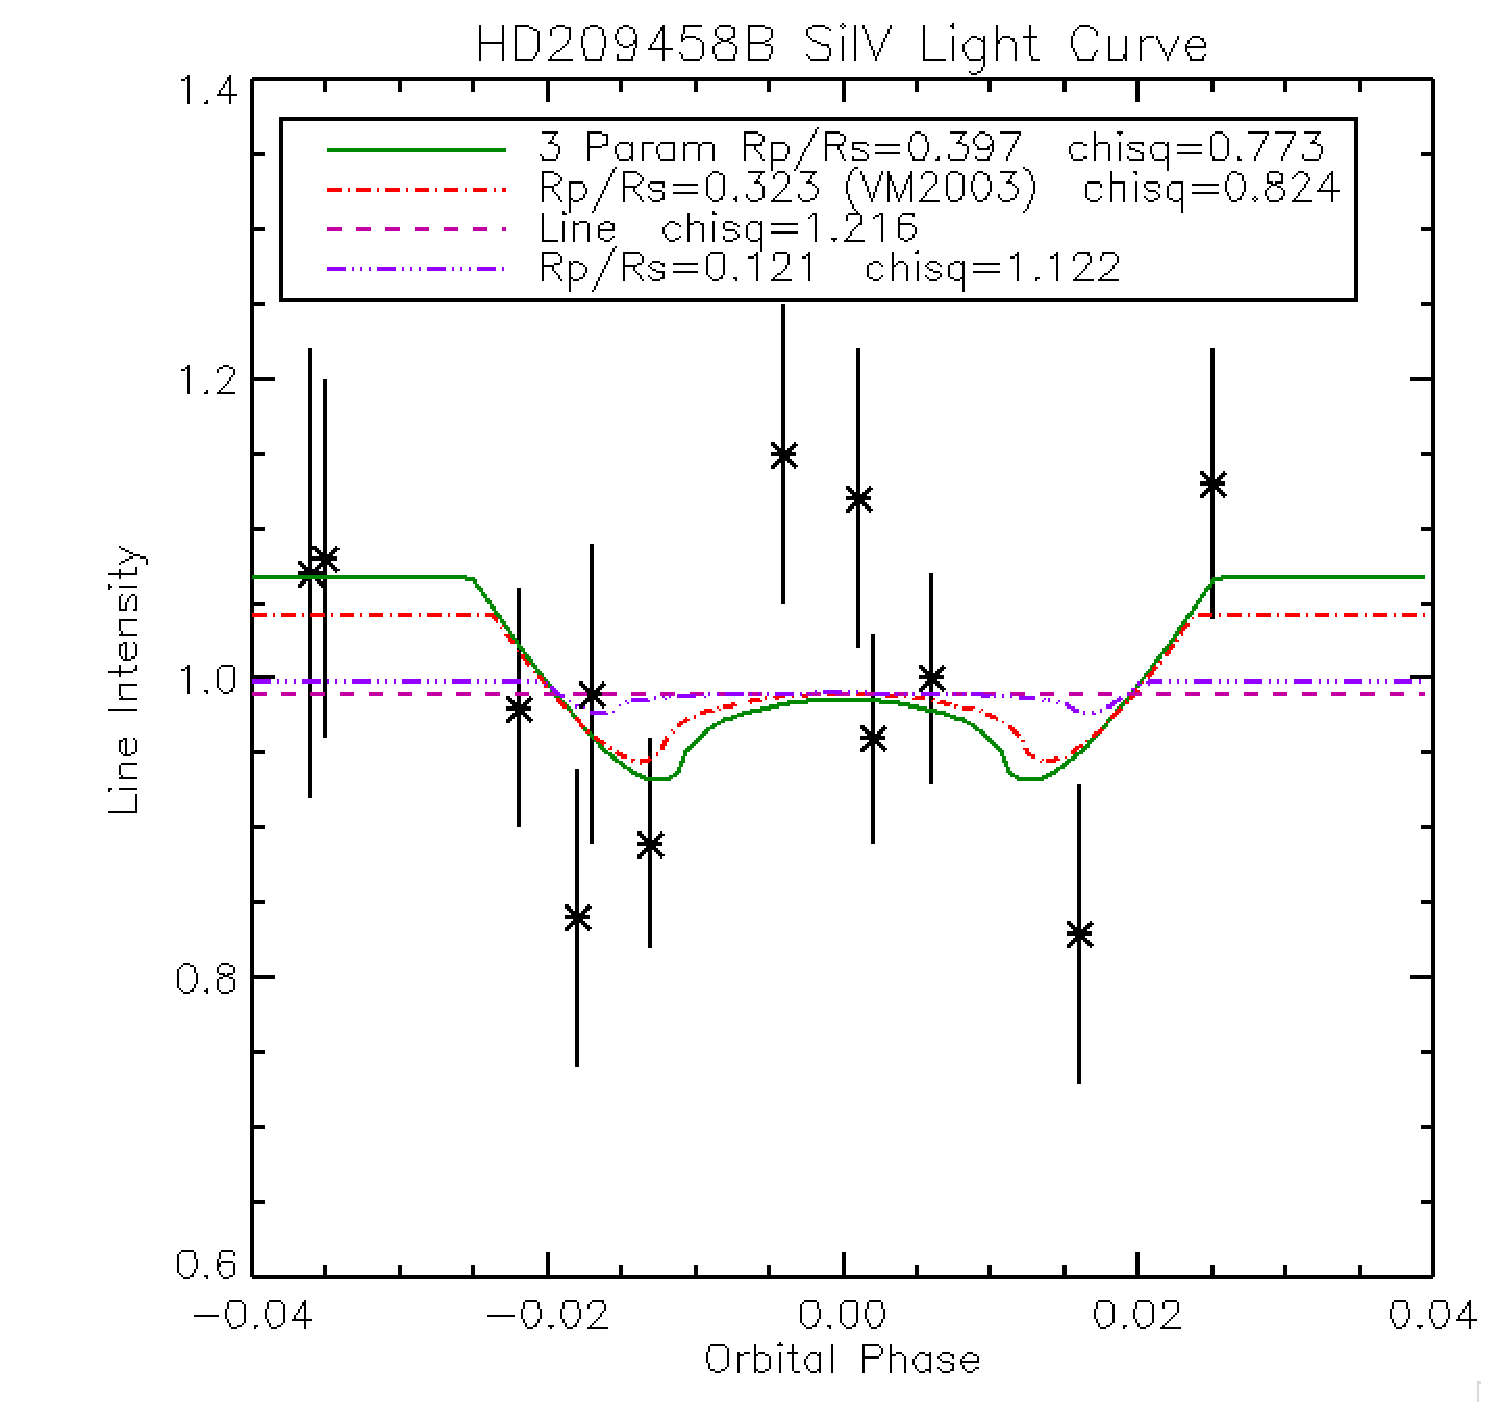
\includegraphics[width=\textwidth]{hd209458.eps}
\caption{Our model fits to the HD 209458b SiIV 1394 \AA\ emission line light curve taken by
  \citet{vidmad}. The 3 parameter fit has the impact parameter, planet
  size and overal height as free parameters. The Levenberg-Marquardt
  model fitting method gives R$_p$/R$_*$ = 0.4 and is given by the
  solid curve. The 
  dash-triple dotted curve is a model where R$_p$/R$_*$ is fixed 1.1,
  as given by optical measurements. For comparison, a line has a normalized
  $\chi^2$ of 1.2 (dashed curve). Also plotted is a model with the
  R$_p$/R$_*$ = 0.3 as found by \citet{vidmad} for the \hi\ and
  \cii\ lines.}
\label{fig03}
\end{figure}

\section{Signal to Noise Calculations} \label{labl:sn}
- What does the NUV flux and (R$_p$/R$_*$) have to be to make this feasible?

\subsection{Chromospheric Science} \label{labl:cscience}
- \\
- In addition to UV transit timing, we could also study chromospheres
- \\
- We can map out spots and even see how they might migrate as done by \citet{2010arXiv1002.4113H}

\section{Conclusion}

\bibliography{paper}
%%  \begin{figure}
%%  \epsscale{.80}
%%  %\plotone{f1.eps}
%%  \caption{Derived spectra for 3C138 \citep[see][]{heiles03}. Plots for all sources are available
%%  in the electronic edition of {\it The Astrophysical Journal}.\label{fig1}}
%%  \end{figure}
%%  
%%  \clearpage
%%  
%%  %% Here we use \plottwo to present two versions of the same figure,
%%  %% one in black and white for print the other in RGB color
%%  %% for online presentation. Note that the caption indicates
%%  %% that a color version of the figure will be available online.
%%  %%
%%  
%%  \begin{figure}
%%  %\plottwo{f2.eps}{f2_color.eps}
%%  \caption{A panel taken from Figure 2 of \citet{rudnick03}. 
%%  See the electronic edition of the Journal for a color version 
%%  of this figure.\label{fig2}}
%%  \end{figure}
%%  
%%  %% This figure uses \includegraphics to scale and rotate the still frame
%%  %% for an mpeg animation.
%%  
%%  \begin{figure}
%%  %\includegraphics[angle=90,scale=.50]{f3.eps}
%%  \caption{Animation still frame taken from \citet{kim03}.
%%  This figure is also available as an mpeg
%%  animation in the electronic edition of the
%%  {\it Astrophysical Journal}.}
%%  \end{figure}
%%  
  \end{document}
%%  
%%  %%
%%  %% End of file `sample.tex'.
